\documentclass{standalone}
\usepackage{pgfplots}

\begin{document}
	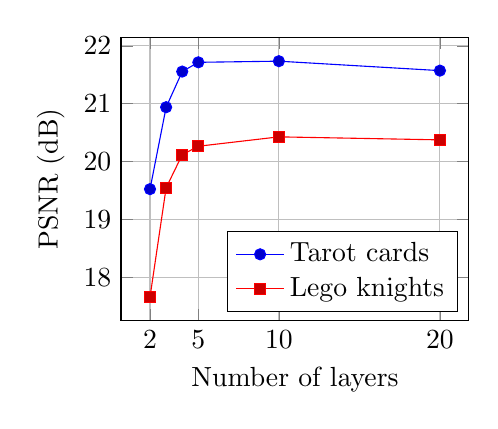
\begin{tikzpicture}
		
		\begin{axis}[	legend pos = south east, 
						legend cell align = left,
						xtick = {2, 5, 10, 20},
						ytick = {18, 19, 20, 21, 22},
						ylabel = {PSNR (dB)},
						xlabel = {Number of layers},
						ylabel near ticks,
						grid,
						axis on top = false,
						width = 6 cm]
						
		%% NOTE: I added the 4.7712 = 10 * log_10(3) because I forgot to normalize the MSE by the number of color channels 
		
			\addplot coordinates {
				(2, 14.7555 + 4.7712)
				(3, 16.1691 + 4.7712)
				(4, 16.7842 + 4.7712)
				(5, 16.9441 + 4.7712)
				(10, 16.9636 + 4.7712)
				(20, 16.8005 + 4.7712)
			};
			\addlegendentry{Tarot cards};
			
			\addplot coordinates {
				(2, 12.8945 + 4.7712)
				(3, 14.7783 + 4.7712)
				(4, 15.3490 + 4.7712)
				(5, 15.4956 + 4.7712)
				(10, 15.6576 + 4.7712)
				(20, 15.6058 + 4.7712)
			};
			\addlegendentry{Lego knights};
			
			 
		\end{axis}
		
	\end{tikzpicture}
\end{document}